\section{MPC Formulation}

\subsection{Overview}
\begin{frame}{Overview}
  How is MPC implemented?\\
  How is the cost function formulated?\\
  How are the constraints implemented?
\end{frame}

\begin{frame}{Quadratic Program}
  How is the QP setup?\\
  What constraints are used?\\
  What type of solver is used?
\end{frame}

\subsection{Distributed MPC}
\begin{frame}{Distributed MPC}
  \begin{figure}[H]
    \centering
    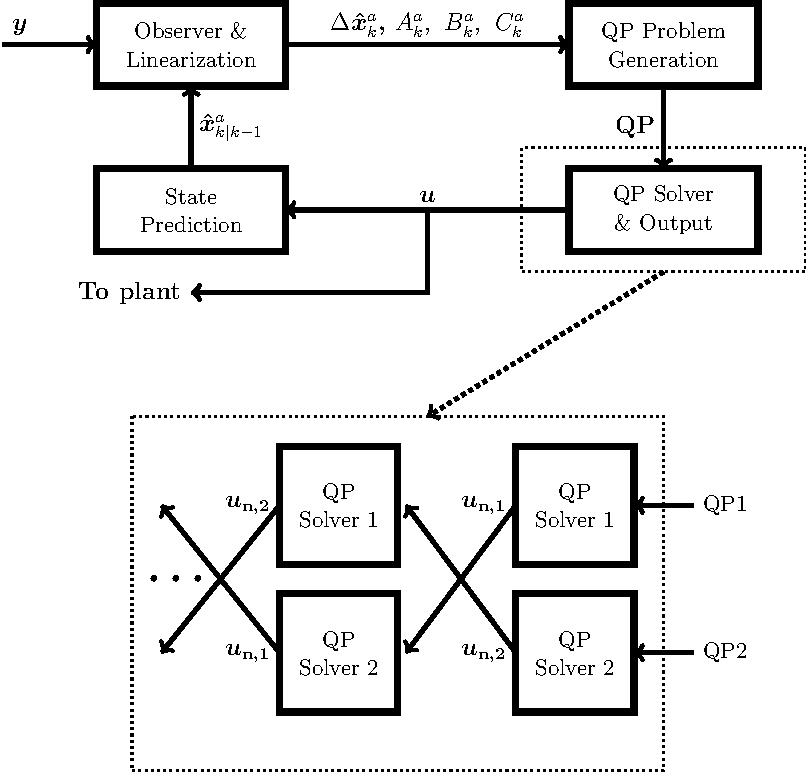
\includegraphics[width=.5\linewidth]{figures/algorithm.pdf}
  \end{figure}
  How does distributed MPC differ from centralized?\\
  How is the cost function set up differently?\\
  What extra terms does it have?
\end{frame}

\subsection{Implementation}
\begin{frame}{State Estimation}
  How are states estimated?\\
  Why a static observer matrix?
\end{frame}

\begin{frame}{Simulink}
  How is the Simulink model set up?\\
  Advantages/disadvantages
\end{frame}

\begin{frame}{C++}
  How is the C++ model set up?\\
  Computational speed advantages?
\end{frame}

